\section{Geometría tridimensional y marcos de referencia}
En la presente sección se presentará la geometría tridimensional y específicamente el concepto de rotación y traslación, junto con algunas de sus representaciones. Si se quiere profundizar en este tema, puede referirse a Barfoot \cite{barfoot2020}.%\textbf{(Barfoot, 2016)}.

Los robots móviles generalmente son libres de trasladarse y rotar. Matemáticamente, tienen seis grados de libertad: tres en traslación y tres en rotación. Esta configuración geométrica de seis grados de libertad se conoce como la \textit{pose} (posición y orientación) del robot. Algunos robots pueden tener múltiples cuerpos conectados entre sí; en este caso cada cuerpo tiene su propia pose. Consideraremos solo el caso de un solo cuerpo en el presente trabajo.

\subsection{Rotaciones}
El vector, $\undervec{r}$, es un objeto geométrico que tiene magnitud y dirección. Este vector puede ser expresado en un \textit{marco de referencia}, $\undervec{\bm{\mathcal{F}}}_a$, como
\begin{align}
    \undervec{r} &= r_1\undervec{a}_1+ r_2\undervec{a}_2 + r_3\undervec{a}_3 \\
    &= 
    \begin{bmatrix}
    r_1 & r_2 & r_3
    \end{bmatrix}
    \begin{bmatrix}
    \undervec{a}_1 \\ 
    \undervec{a}_2 \\
    \undervec{a}_3
    \end{bmatrix}
    \\
    &= \bm{r}_a^T\undervec{\bm{\mathcal{F}}}_a
\end{align}
donde $\undervec{\bm{\mathcal{F}}}_a$ contiene a los \textit{vectores base}, formando así el marco de referencia $a$, mientras que $\bm{r}_a$ es una matriz columna que contiene los \textit{componentes} o \textit{coordenadas} de $\undervec{r}$ en el marco de referencia $\undervec{\bm{\mathcal{F}}}_a$. De forma análoga, el vector $\undervec{r}$ puede ser escrito como
\begin{equation}
    \undervec{r} = \undervec{\bm{\mathcal{F}}}_a^T \bm{r}_a
\end{equation}

\subsubsection{Matriz de rotación}
Si se quisiera expresar al vector $\undervec{r}$ para dos marcos de coordenadas distintos, como puede verse en la Figura \ref{fig:rotatedcoordinateframes}, para cada uno de los marcos dicho vector será representado como
\begin{align}
    \undervec{\bm{\mathcal{F}}}_a &\rightarrow \bm{r}_a \\
    \undervec{\bm{\mathcal{F}}}_b &\rightarrow \bm{r}_b
\end{align}
% \begin{figure}
%     \centering
%     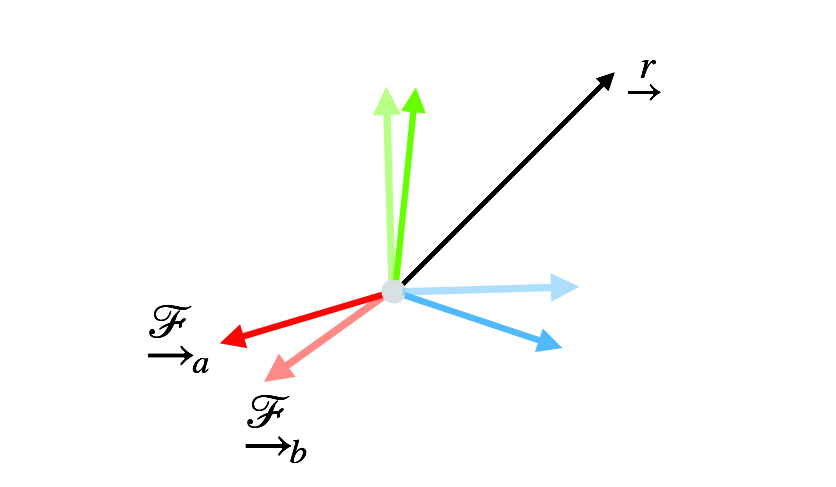
\includegraphics[width=\textwidth]{Img/RotatedCoordinateFrames.png}
%     \caption{Dos marcos de coordenadas con un vector en el espacio fijo}
%     \label{fig:rotatedcoordinateframes_old}
% \end{figure}

\begin{figure}
    \centering
    \tdplotsetmaincoords{50}{140}
\begin{tikzpicture}[scale=4,baseline,tdplot_main_coords]
    \coordinate (O) at (0,0,0);
    
    \draw[thick,->] (0,0,0) -- (1,0,0) node[anchor=north west]{$\undervec{\bm{\mathcal{F}}}_a$};
    \draw[thick,->] (0,0,0) -- (0,1,0);
    \draw[thick,->] (0,0,0) -- (0,0,1);
    
    \draw[thick,->,blue] (0,0,0) -- (0,1,1) node[anchor=north west]{$\undervec{\bm{r}}$};
    
    \pgfmathsetmacro{\ax}{2}
    \pgfmathsetmacro{\ay}{2}
    \pgfmathsetmacro{\az}{1}
    
    \tdplotsetrotatedcoords{20}{20}{0}
    
    \draw[->,tdplot_rotated_coords,red] (0,0,0) -- (.7,0,0) node[anchor=north west]{$\undervec{\bm{\mathcal{F}}}_b$};
    \draw[->,tdplot_rotated_coords,red] (0,0,0) -- (0,.8,0);
    \draw[->,tdplot_rotated_coords,red] (0,0,0) -- (0,0,1.2);
    
    \tdplotgetpolarcoords{\ax}{\ay}{\az}
    
    \tdplotsetthetaplanecoords{\tdplotresphi}
    
    
\end{tikzpicture}
    \caption{Dos marcos de coordenadas con un vector en el espacio fijo}
    \label{fig:rotatedcoordinateframes}
\end{figure}


Ya que para este caso el origen de ambos marcos es el mismo, las coordenadas del vector están relacionadas mediante una \textit{matriz de rotación}
\begin{equation}
    \bm{r}_b = \bm{C}_{ba}\bm{r}_a
\end{equation}
donde
\begin{align}
    \bm{C}_{ba} &= \undervec{\bm{\mathcal{F}}}_b\cdot \undervec{\bm{\mathcal{F}}}_a^T \\
    &=
    \begin{bmatrix}
    \undervec{b}_1 \\
    \undervec{b}_2 \\
    \undervec{b}_3 \\
    \end{bmatrix}
    \cdot
    \begin{bmatrix}
    \undervec{a}_1 & \undervec{a}_2 & \undervec{a}_3
    \end{bmatrix} \\
    &=
    \begin{bmatrix}
    \undervec{b}_1 \cdot \undervec{a}_1 & \undervec{b}_1 \cdot \undervec{a}_2 & \undervec{b}_1 \cdot \undervec{a}_3 \\
    \undervec{b}_2 \cdot \undervec{a}_1 & \undervec{b}_2 \cdot \undervec{a}_2 & \undervec{b}_2 \cdot \undervec{a}_3 \\
    \undervec{b}_3 \cdot \undervec{a}_1 & \undervec{b}_3 \cdot \undervec{a}_2 & \undervec{b}_3 \cdot \undervec{a}_3
    \end{bmatrix}
\end{align}
siendo $\cdot$ el \textit{producto escalar} o \textit{producto interno}, esta matriz toma las coordenadas en el marco $a$ y las gira en el marco $b$. Estas matrices tienen como característica de ser \textit{ortonormales}, ya que su inversa es equivalente a su transpuesta. Por lo tanto, se cumple que
\begin{equation}
    \bm{C}_{ba}\bm{C}_{ba}^T = \bm{C}_{ba}\bm{C}_{ab} = 1
\end{equation}

Si, por ejemplo, se tuviesen tres marcos de referencia, $\undervec{\bm{\mathcal{F}}}_a$, $\undervec{\bm{\mathcal{F}}}_b$, $\undervec{\bm{\mathcal{F}}}_c$, con las componentes de cada uno para representar al vector $\undervec{r}$ siendo $\bm{r}_a$, $\bm{r}_b$ y $\bm{r}_c$ respectivamente, entonces
\begin{equation}
    \bm{r}_c = \bm{C}_{cb}\bm{r}_b = \bm{C}_{cb}\bm{C}_{ba}\bm{r}_a
\end{equation}
y como $\bm{r}_c = \bm{C}_{ca}\bm{r}_a$, entonces
\begin{equation}
    \bm{C}_{ca} = \bm{C}_{cb}\bm{C}_{ba}
\end{equation}{}

La matriz de rotación describe la orientación tanto global como única. Esto requiere nueve parámetros, los cuales no son independientes. Sin embargo, existen otras alternativas a la hora de representar una orientación de un marco de referencia respecto a otro.

\subsubsection{Rotaciones principales}
Antes de entrar en rotaciones más complejas, hay que tomar por caso las rotaciones elementales, o sea, las que se efectúan tomando un eje de coordenadas. La situación donde $\undervec{\bm{\mathcal{F}}}_b$ ha sido rotado de $\undervec{\bm{\mathcal{F}}}_a$ a través de una rotación sobre los tres ejes, lo que puede observarse en la Figura \ref{fig:rotations}.

% \begin{figure}[!h]
%     \centering
%     \subfloat[Rotación alrededor de $z$]{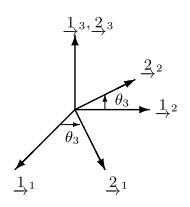
\includegraphics[width=.33\textwidth]{Img/RotationInX.png}}
%     \hfill
%     \subfloat[Rotación alrededor de $y$]{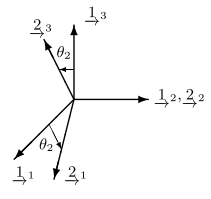
\includegraphics[width=.33\textwidth]{Img/RotationInY.png}}
%     \hfill
%     \subfloat[Rotación alrededor de $x$]{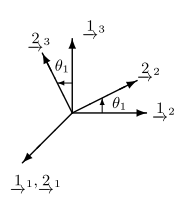
\includegraphics[width=.33\textwidth]{Img/RotationInZ.png}}
%     \caption{Rotaciones principales}
%     \label{fig:rotations_old}
% \end{figure}

\begin{figure}
    \centering
    \subfloat[Rotación alrededor de $x$]{\tdplotsetmaincoords{50}{140}
\begin{tikzpicture}[scale=2,tdplot_main_coords]
    \draw[thick,->] (0,0,0) -- (1,0,0) node[anchor=north east]{$x$};
    \draw[thick,->] (0,0,0) -- (0,1,0) node[anchor=north west]{$y$};
    \draw[thick,->] (0,0,0) -- (0,0,1) node[anchor=south]{$z$};
    
    \pgfmathsetmacro{\ax}{-.75}
    \pgfmathsetmacro{\ay}{2.5}
    \pgfmathsetmacro{\az}{0}
    
    \tdplotsetrotatedcoords{20}{40}{00}
    
    \draw[thick,color=red,tdplot_rotated_coords,->] (0,0,0) -- (.7,0,0) node[anchor=east]{$x’$};
    \draw[thick,color=green!50!black,tdplot_rotated_coords,->] (0,0,0) -- (0,.7,0) node[anchor=west]{$y’$};
    \draw[thick,color=blue,tdplot_rotated_coords,->] (0,0,0) -- (0,0,.7) node[anchor=south]{$z’$};
    
    \tdplottransformrotmain{\ax}{\ay}{\az}
    
    \draw[tdplot_main_coords,->,blue!50] (0,0,0) -- (\tdplotresx,\tdplotresy,\tdplotresz);
    \node[tdplot_rotated_coords,anchor=north] at (\ax,\ay,\az){Rotated coords: (\ax, \ay, \az)};
    \node[tdplot_main_coords,anchor=south] at (\tdplotresx,\tdplotresy,\tdplotresz){Main coords: (\tdplotresx, \tdplotresy, \tdplotresz)};

\end{tikzpicture}}
    \quad
    \subfloat[Rotación alrededor de $y$]{\tdplotsetmaincoords{50}{140}
\begin{tikzpicture}[scale=4,baseline,tdplot_main_coords]
    \coordinate (O) at (0,0,0);
    
    \draw[thick,->] (0,0,0) -- (1,0,0) node[anchor=north west]{$x$};
    \draw[thick,->] (0,0,0) -- (0,1,0) node[anchor=north west]{$y$};
    \draw[thick,->] (0,0,0) -- (0,0,1) node[anchor=north west]{$z$};
    
    \pgfmathsetmacro{\ax}{2}
    \pgfmathsetmacro{\ay}{2}
    \pgfmathsetmacro{\az}{1}
    
    \tdplotsetrotatedcoords{20}{20}{0}
    
    \draw[->,tdplot_rotated_coords,red] (0,0,0) -- (.7,0,0) node[anchor=south]{$x'$};
    \draw[->,red] (0,0,0) -- (0,1,0) node[anchor=north east]{$y'$};
    \draw[->,tdplot_rotated_coords,red] (0,0,0) -- (0,0,1) node[anchor=north east]{$z'$};
    
    \tdplotgetpolarcoords{\ax}{\ay}{\az}
    
    \tdplotsetthetaplanecoords{\tdplotresphi}
    
    % \tdplotdrawarc[tdplot_rotated_coords]{(0,0,0)}{1}{0}%
    % % tdplotdrawarc[tdplot_rotated_coords]{(0,0,0)}{1}{0}%
    % {\tdplotrestheta}{anchor=west}{$\theta = \tdplotrestheta$}
    \tdplotdrawarc{(0,0,0)}{0.5}{230}{241}{anchor=south}{$\theta_2$}
    \tdplotdrawarc{(0,0,0)}{0.5}{0}{30}{anchor=north east}{$\theta_2$}
    
\end{tikzpicture}}
    \quad
    \subfloat[Rotación alrededor de $z$]{\tdplotsetmaincoords{50}{140}
\begin{tikzpicture}[scale=4,baseline,tdplot_main_coords]
    \coordinate (O) at (0,0,0);
    
    \draw[thick,->] (0,0,0) -- (1,0,0) node[anchor=north east]{$x$};
    \draw[thick,->] (0,0,0) -- (0,1,0) node[anchor=north west]{$y$};
    \draw[thick,->] (0,0,0) -- (0,0,1) node[anchor=north west]{$z$};
    
    \pgfmathsetmacro{\ax}{2}
    \pgfmathsetmacro{\ay}{2}
    \pgfmathsetmacro{\az}{1}
    
    \tdplotsetrotatedcoords{20}{20}{0}
    
    \draw[->,tdplot_rotated_coords,red] (0,0,0) -- (.7,0,0) node[anchor=north east]{$x'$};
    \draw[->,tdplot_rotated_coords,red] (0,0,0) -- (0,.7,0) node[anchor=north west]{$y'$};
    \draw[->,red] (0,0,0) -- (0,0,\az) node[anchor=north east]{$z'$};
    
    \tdplotgetpolarcoords{\ax}{\ay}{\az}
    
    \tdplotsetthetaplanecoords{\tdplotresphi}
    
    % \tdplotdrawarc[tdplot_rotated_coords]{(0,0,0)}{1}{0}%
    % % tdplotdrawarc[tdplot_rotated_coords]{(0,0,0)}{1}{0}%
    % {\tdplotrestheta}{anchor=west}{$\theta = \tdplotrestheta$}
    \tdplotdrawarc{(0,0,0)}{0.5}{0}{30}{anchor=north}{$\theta_3$}
    \tdplotdrawarc{(0,0,0)}{0.5}{90}{110}{anchor=north west}{$\theta_3$}
    
\end{tikzpicture}}
    \caption{Rotaciones principales}
    \quad
    \label{fig:rotations}
\end{figure}

La matriz de rotación para el caso de la Figura \ref{fig:rotations}.a, el cual corresponde a una sobre el eje $x$, es
\begin{equation}
    \bm{C}_1 = 
    \begin{bmatrix}
        1 & 0 & 0 \\
        0 & \cos \theta_1 & \sin \theta_1 \\
        0 & -\sin \theta_1 & \cos \theta_1
    \end{bmatrix}
\end{equation}

En cambio, la matriz de rotación para el eje $y$, como se aprecia en la Figura \ref{fig:rotations}.b,
\begin{equation}
    \bm{C}_2 = 
    \begin{bmatrix}
        \cos \theta_2 & 0 & - \sin \theta_2 \\
        0 & 1 & 0 \\
        \sin \theta_2 & 0 & \cos \theta_2
    \end{bmatrix}
\end{equation}

Finalmente, la rotación en $z$ vista en la Figura \ref{fig:rotations}.c

\begin{equation}
    \bm{C}_3 = 
    \begin{bmatrix}
        \cos \theta_3 & \sin \theta_3 & 0 \\
        -\sin \theta_3 & \cos \theta_3 & 0 \\
        0 & 0 & 1
    \end{bmatrix}
\end{equation}


\subsubsection{Ángulos de Euler}
La orientación de un marco de referencia respecto a otro puede, también, ser especificada como una secuencia de tres rotaciones principales. Dependiendo el orden con el que se hagan dichas rotaciones, se conseguirán resultados distintos. Esto es debido a que las rotaciones en tres dimensiones no pertenecen a un espacio vectorial (y, por lo tanto, no pueden ser representadas por una), y suele considerárselas como un \textit{grupo}, el cual es una abstracción matemática. %Existen dentro de la literatura numerosos textos que tratan el tema, como pueden ser \textbf{PONER COSAS QUE HABLEN DE SO(3) SU(2) ETC ETC}.

En concreto, una secuencia muy utilizada en aplicaciones aeroespaciales realiza
\begin{enumerate}
    \item Una rotación $\theta_1$ sobre el eje original $1$ (rotación en ''roll'')
    \item Una rotación $\theta_2$ sobre el eje intermedio $2$ (rotación en ''pitch'')
    \item Una rotación $\theta_3$ sobre el eje transformado $3$ (rotación en ''yaw'')
\end{enumerate}
la cual suele ser llamada la secuencia 1-2-3 de actitud o la convención ''roll-pitch-yaw''. En este caso, la matriz de rotación del marco 1 al marco 2 está dada por
\begin{align}
    \bm{C}_{21}(\theta_3,\theta_2,\theta_1) &= \bm{C}_3(\theta_3)\bm{C}_2(\theta_2)\bm{C}_1(\theta_1) \\
    &=
    \begin{bmatrix}
        c_2c_3 & c_1s_3+s_1s_2c_3 & s_1s_3 - c_1s_2c_3 \\
        -c_2s_3 & c_1c_3 - s_1s_2s_3 & s_1c_3 + c_1s_2s_3 \\
        s_2 & -s_1c_2 & c_1c_2
    \end{bmatrix}
    \label{eq:rpyrotation}
\end{align}
donde $s_i = \sin{\theta_i}$ y $c_i = \cos{\theta_i}$.

Todas las secuencias de Euler tienen singularidades. Para la secuencia 1-2-3, una singularidad existe en $\theta_2 = \pi/2$. En este caso,

\begin{equation}
    \bm{C}_{21}(\theta_3,\frac{\pi}{2},\theta_1) = 
    \begin{bmatrix}
        0 & \sin{(\theta_1 + \theta_3)} & -\cos{(\theta_1 + \theta_3)} \\
        0 & \cos{(\theta_1 + \theta_3)} & \sin{(\theta_1 + \theta_3)} \\
        1 & 0 & 0
    \end{bmatrix}
\end{equation}

Por lo tanto, $\theta_1$ y $\theta_3$ se asocian con la misma rotación. Sin embargo, esto es solo un problema si se quieren recuperar los ángulos de  rotación de la matriz de rotación.

\paragraph{Rotaciones infinitesimales} Si los ángulos $\theta_1$, $\theta_2$, $\theta_3$ son pequeños, puede aproximarse que $c_i \approx 1$, $s_i \approx \theta_i$ y que, por ende, $\theta_i\theta_j$ es despreciable respecto a $1$. Entonces, para la transformación 1-2-3, la Expresión (\ref{eq:rpyrotation}) resulta
\begin{equation}
    \bm{C}_{21} \approx
    \begin{bmatrix}
        1 & \theta_3 + \theta_1\theta_2 & \theta_1\theta_3 - \theta_2 \\
        -\theta_3 & 1 & \theta_1 + \theta_2\theta_3 \\
        \theta_2 & -\theta_1 & 1
    \end{bmatrix}
    \label{eq:rpyinfinitesimal}
\end{equation}
ya que $\theta_1\theta_2$ es despreciable respecto a $1$.

Si además se desprecian los productos de ángulos pequeños $\theta_i\theta_j \approx 0$
\begin{align}
    \bm{C}_{21} &\approx
    \begin{bmatrix}
        1 & \theta_3 & -\theta_2 \\
        -\theta_3 & 1 & \theta_1 \\
        \theta_2 & -\theta_1 & 1
    \end{bmatrix}
    \label{eq:rpyinfinitesimalreduced}
    \\
    &\approx \bm{1} - \left[\bm{\theta}\right]_\times
\end{align}
siendo $\bm{\theta}$ el \textit{vector de rotación}, donde
\begin{align}
    \bm{\theta} &=
    \begin{bmatrix}
        \theta_1 \\
        \theta_2 \\
        \theta_3
    \end{bmatrix}
    \\
    \left[\bm{a}\right]_\times &= 
    \begin{bmatrix}
        0 & -a_z & a_y \\
        a_z & 0 & -a_x \\
        -a_y & a_x & 0
    \end{bmatrix}
\end{align}

\subsubsection{Cuaterniones}
Un cuaternión es una extensión de los números complejos, con tres raíces cuadradas de $-1$ ($ijk$) en lugar de solo una ($i$). Un cuaternión puede ser representado como un vector cuatridimensional de longitud unitaria, donde la primer componente es un número escalar real, mientras que las otras tres componentes forman un vector en el espacio $ijk$ siguiendo la regla de la mano derecha. 
\begin{equation}
    \bm{q} = q_w + q_i i + q_j j + q_k = q_w k = q_w \bm{q}_v
\end{equation}
siendo $q_w$ la \textit{parte real} y $\bm{q}_v$ a la \textit{parte vectorial}, cumpliéndose que
\begin{equation}
    i^2=j^2=k^2=ijk=-1
\end{equation}

Usualmente, se representa al mismo como un vector $\bm{q}$ de cuatro componentes
\begin{equation}
    \bm{q} =
    \begin{bmatrix}
    q_w \\
    \bm{q}_v
    \end{bmatrix}
\end{equation}
y al ser de interés en este trabajo los cuaterniones para expresar rotaciones, los mismos son \textit{unitarios} o \textit{normalizados}
\begin{align}
    \bm{q}(\hat{\bm{u}},\phi) =
    \begin{bmatrix}
    q_w(\phi) \\
    \bm{q}_v(\hat{\bm{u}},\phi)
    \end{bmatrix}
    &=
    \begin{bmatrix}
        \cos{\frac{\phi}{2}} \\
        \hat{\bm{u}}\sin{\frac{\phi}{2}}
    \end{bmatrix}
    \\
    ||\bm{q}(\hat{\bm{u}},\phi)|| &= 1
\end{align}

% \textbf{PONER O NO ESTO?????}
% En otras palabras, dicho cuaternión parametriza una rotación sobre un eje definido por el vector $\hat{\bm{u}}$, y un ángulo $\phi$ sobre ese vector, como puede verse en la Figura \ref{fig:quaternions}.
% \begin{figure}
%     \centering
%     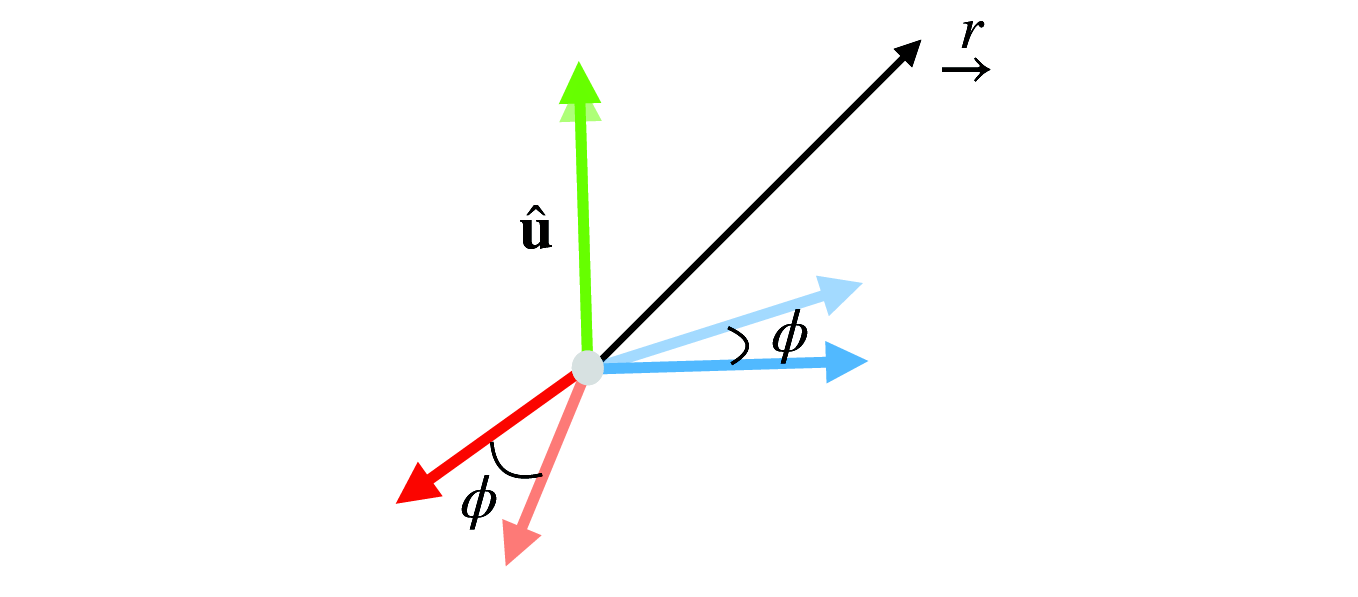
\includegraphics[width=\textwidth]{Img/Quaternions.png}
%     \caption{Rotación sobre un eje definido?}
%     \label{fig:quaternions}
% \end{figure}

\paragraph{Propiedades de los cuaterniones}
A continuación, se evaluarán algunas de las propiedades de los cuaterniones.
\subparagraph{Suma}
Tanto la suma como la resta son de forma directa
\begin{equation}
    \bm{p} \pm \bm{q} =
    \begin{bmatrix}
        p_w + q_w \\
        \bm{p}_v + \bm{q}_v
    \end{bmatrix}
\end{equation}

La suma, entonces, es \textit{conmutativa} y \textit{asociativa}
\begin{align}
    \bm{p} + \bm{q} &= \bm{q} + \bm{p} \\
    \bm{p} + (\bm{q} + \bm{s}) &= (\bm{p} + \bm{q}) + \bm{s}
\end{align}

\subparagraph{Producto}
Denotado con $\otimes$, el producto resulta
\begin{equation}
    \bm{p}\otimes\bm{q} = 
    \begin{bmatrix}
        p_wq_w - p_xq_x - p_yq_y - p_zq_z \\
        p_wq_x + p_xq_w + p_yq_z - p_zq_y \\
        p_wq_y - p_xq_z + p_yq_w + p_zq_x \\
        p_wq_z + p_xq_y - p_yq_x + p_zq_w
    \end{bmatrix}
\end{equation}

Por inspección, puede escribirse como un producto matricial
\begin{align}
    \bm{p}\otimes\bm{q} &= 
    \begin{bmatrix}
        q_w & -q_x & -q_y & -q_z \\
        q_x & q_w & q_z & -q_y \\
        q_y & -q_z & q_w & q_x \\
        q_z & q_y & -q_x & q_w
    \end{bmatrix}
    \begin{bmatrix}
        p_w \\
        p_x \\
        p_y \\
        p_z
    \end{bmatrix}
    \\
    &= 
    [\bm{q}]_R \bm{p}
    \label{eq:quaternionproductright}
\end{align}
y de forma análoga
\begin{align}
    \bm{p}\otimes\bm{q} &= 
    \begin{bmatrix}
        p_w & -p_x & -p_y & -p_z \\
        p_x & p_w & -p_z & p_y \\
        p_y & p_z & p_w & -p_x \\
        p_z & -p_y & p_x & p_w
    \end{bmatrix}
    \begin{bmatrix}
        q_w \\
        q_x \\
        q_y \\
        q_z
    \end{bmatrix}
    \\
    &= [\bm{p}]_L\bm{q}
    \label{eq:quaternionproductleft}
\end{align}
donde se definen a las matrices de producto de cuaterniones izquierda y derecha como
\begin{align}
    [\bm{q}]_R &= q_w\bm{I} +
    \begin{bmatrix}
        0 & -\bm{q_v}^T \\
        \bm{q}_v & -[\bm{q}_v]_\times
    \end{bmatrix}
    \label{eq:quaternionproductmatrixright}
    \\
    [\bm{q}]_L &= q_w\bm{I} +
    \begin{bmatrix}
        0 & -\bm{q_v}^T \\
        \bm{q}_v & [\bm{q}_v]_\times
    \end{bmatrix}
    \label{eq:quaternionproductmatrixleft}
\end{align}

El producto, entonces, es \textit{no conmutativo} en el caso general. Sin embargo, es \textit{asociativo}, además de \textit{distributivo sobre la suma}
\begin{align}
    \bm{p}\otimes\bm{q} &\neq \bm{q}\otimes\bm{p} \\
    (\bm{p}\otimes\bm{q})\otimes\bm{s} &= \bm{p}\otimes(\bm{q}\otimes\bm{s}) \\
    \bm{p}\otimes(\bm{q} + \bm{s}) &= \bm{p}\otimes\bm{q} + \bm{p}\otimes\bm{s} \\
    (\bm{p} + \bm{q})\otimes\bm{s} &= \bm{p}\otimes\bm{s} + \bm{q}\otimes\bm{s}
\end{align}
\subparagraph{Conjugado}
El conjugado de un cuaternión se define como
\begin{equation}
    \bm{q}^* = q_w - \bm{q_v}
\end{equation}
y tiene las propiedades de
\begin{align}
    \bm{q}\otimes\bm{q}^* = \bm{q^*}\otimes\bm{q} &= q_w^2 + q_x^2 + q_y^2 + q_z^2 \\
    (\bm{p}\otimes\bm{q})^* &= \bm{q}^*\otimes\bm{p}^*
\end{align}

\subparagraph{Norma}
La norma se define como
\begin{equation}
    ||\bm{q}|| = \sqrt{\bm{q}\otimes\bm{q}^*} = \sqrt{q_w^2 + q_x^2 + q_y^2 + q_z^2}
\end{equation}
y tiene la propiedad de
\begin{equation}
    ||\bm{p}\otimes\bm{q}|| = ||\bm{q}\otimes\bm{p}|| = ||\bm{p}|| \ ||\bm{q}||
\end{equation}

\subparagraph{Inversa}
La inversa de un cuaternión es aquella que si se realiza la multiplicación del cuaternion con la misma se obtiene la identidad.
\begin{equation}
    \bm{q}\otimes\bm{q}^{-1} = \bm{q}^{-1}\otimes\bm{q} = 1
    \label{eq:quaternioninverse}
\end{equation}
cuya expresión es
\begin{equation}
    \bm{q}^{-1} = \frac{\bm{q}^*}{||\bm{q}||^2}
\end{equation}

Si se trata de un \textit{cuaternión unitario}, esto es, $||\bm{q}|| = 1$, entonces
\begin{equation}
    \bm{q}^{-1} = \bm{q}^*    
\end{equation}

\subparagraph{Conmutador}
El \textit{conmutador} de un cuaternión se define como
\begin{equation}
    [\bm{p},\bm{q}] = \bm{p}\otimes\bm{q} - \bm{q}\otimes\bm{p} = \bm{p}_v\otimes\bm{q}_v - \bm{q}_v\otimes\bm{p}_v = 2\bm{p}_v\times\bm{q}_v
    \label{eq:quaternioncommutator}
\end{equation}

\paragraph{Rotaciones con cuaterniones}
Si se tiene un vector en el marco $a$ definido como $\bm{r}_a$, y al mismo se lo quiere llevar al marco $b$, del cual solo se diferencia por una rotación, esto puede hacerse con un cuaternión $\bm{q}$ que describa esa rotación mediante
\begin{equation}
    \bm{r}_b = \bm{q}\otimes\bm{r}_a\otimes\bm{q}^{-1}
    \label{eq:quaternionvectorrotation}
\end{equation}
donde tanto $\bm{r}_a$ como $\bm{r}_b$ corresponden a los vectores expresados en su forma de cuaternión, esto es,
\begin{equation}
    \bm{r} = 
    \begin{bmatrix}
    0 \\
    \bm{r}
    \end{bmatrix}
    \label{eq:vectorquaternionform}
\end{equation}

De forma análoga, puede convertirse un cuaternión a una matriz de rotación utilizando
\begin{align}
    \bm{r}_b &= \bm{C}(\bm{q}_{ba})\bm{r}_a \\
    \bm{C}(\bm{q}) &= (q_w^2 - \bm{q}_v^T\bm{q}_v)\bm{1} + 2\bm{q}_v\bm{q}_v^T + 2q_w\left[\bm{q}_v\right]_\times
\end{align}

\subsubsection{Resumen}
El punto principal para darse cuenta de las diferentes representaciones de las rotaciones es que siempre hay solo tres grados de libertad. Aquellas que tienen más de tres parámetros deben tener restricciones asociadas para limitar el número de grados de libertad a tres. Las representaciones que tienen exactamente tres parámetros tienen singularidades asociadas. No existe una representación perfecta que sea mínima (es decir, que tenga solo tres parámetros) y que también esté libre de singularidades\cite{stuelpnagle1964}.% \textbf{[Stuelpnagel, 1964]}.

De las tres representaciones vistas, esto es, la \textit{matriz de rotación}, los \textit{ángulos de Euler} y los \textit{cuaterniones}, cada una tiene ventajas como desventajas, reflejadas en la Tabla (\ref{tab:rotationrepresentations}).

\begin{table}[!ht]
\centering
\begin{tabular}{c|c|c|c}
                        & \textbf{\begin{tabular}[c]{@{}c@{}}Matriz \\ de rotación\end{tabular}} &  \textbf{\begin{tabular}[c]{@{}c@{}}Ángulos \\ de Euler\end{tabular}} & \textbf{Cuaterniones} \\ \hline \hline
\textit{Expresión}      & $\bm{C}$   & $\{\theta_3,\theta_2,\theta_1\}$     & $\bm{q} = 
    \begin{bmatrix}
        \cos{\frac{\phi}{2}} \\
        \hat{\bm{u}}\sin{\frac{\phi}{2}}
    \end{bmatrix}$  \\ \hline
\textit{Parámetros}     & 9          & 3                  & 4                                             \\ \hline 
\textit{Restricciones}  & $\bm{C}\bm{C}^T = \bm{1}$ &    No & $||\bm{q}|| = 1$                        \\ \hline 
\textit{Singularidades} & No             & Si                       
              & No                   \end{tabular}
\caption{Resumen de las representaciones de rotaciones vistas}
\label{tab:rotationrepresentations}
\end{table}

\subsection{Poses}
Como se ha hablado anteriormente a la rotación, ahora se presenta a la notación de \textit{traslación}. Juntos, la traslación y rotación de un cuerpo se denomina \textit{pose}. Los problemas de estimación de la pose a menudo tienen que ver con la transformación de las coordenadas de un punto, $P$, entre un marco de vehículo en movimiento (en traslación y rotación) y un marco estacionario, como se muestra en la Figura \ref{fig:pose}.
% \begin{figure}[!b]
%     \centering
%     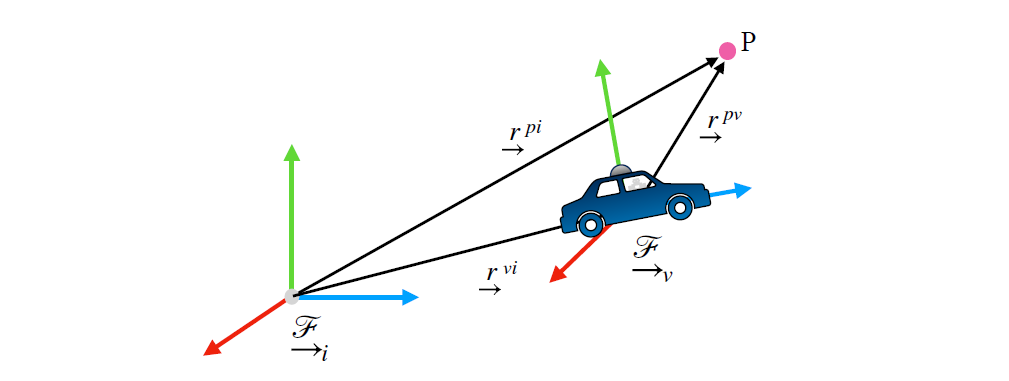
\includegraphics[width=\textwidth]{Img/Pose.png}
%     \caption{Estimación de la pose de un vehículo}
%     \label{fig:pose_old}
% \end{figure}

\begin{figure}
    \centering
    \tdplotsetmaincoords{60}{110}
\begin{tikzpicture}[scale=4,baseline,tdplot_main_coords]
    \draw[thick,->] (0,0,0) -- (.7,0,0) node[anchor=north east]{$\undervec{\bm{\mathcal{F}}}_i$};
    \draw[thick,->] (0,0,0) -- (0,.7,0);
    \draw[thick,->] (0,0,0) -- (0,0,.7);
    
    \coordinate (Shift) at (1,1.5,1);
    \coordinate (Point) at (2,2.4,3);
    \draw[thick,->,blue] (0,0,0) -- (Shift) node[midway,anchor=north west]{$\undervec{\bm{r}}^{vi}$};
    
    
    \draw[thick,->,blue] (0,0,0) -- (Point) node[midway,anchor=south east]{$\undervec{\bm{r}}^{pi}$};
    
    \draw[thick,->,blue] (Shift) -- (Point) node[midway,anchor=north west]{$\undervec{\bm{r}}^{pv}$};
    
    \draw[fill=black] (Point) circle (0.03) node[above right] {$p$};
    \tdplotsetrotatedcoords{20}{-10}{10}
    
    \tdplotsetrotatedcoordsorigin{(Shift)}
    
    \draw[thick,color=red,tdplot_rotated_coords,->] (0,0,0)-- (1,0,0) node[anchor=north east]{$\undervec{\bm{\mathcal{F}}}_v$};
    \draw[thick,color=red,tdplot_rotated_coords,->] (0,0,0)-- (0,.7,0);
    \draw[thick,color=red,tdplot_rotated_coords,->] (0,0,0)-- (0,0,.7);
    
\end{tikzpicture}
    \caption{Estimación de la pose de un vehículo}
    \label{fig:pose}
\end{figure}

Pueden relacionarse los vectores de dicha Figura como
\begin{equation}
    \undervec{r}^{pi} = \undervec{r}^{pv}+\undervec{r}^{vi}
\end{equation}
donde no fue elegido todavía ningún marco de referencia particular en el cual expresar la relación. Escribiendo la relación en el marco estacionario, $\undervec{\bm{\mathcal{F}}}_i$, se tiene
\begin{equation}
    \bm{r}_i^{pi} = \bm{r}_i^{pv} + \bm{r}_i^{vi}
\end{equation}

Si el punto $P$ se encuentra adjunto al vehículo, se conocen típicamente sus coordenadas en $\undervec{\bm{\mathcal{F}}}_v$, el cual está rotado respecto a $\undervec{\bm{\mathcal{F}}}_i$. Siendo $\bm{C}_{iv}$ la representación de esta rotación, puede reescribirse la relación como
\begin{equation}
    \bm{r}_i^{pi} = \bm{C}_{iv}\bm{r}_v^{pv} + \bm{r}_i^{vi}
    \label{eq:poseconvertion}
\end{equation}
que indica cómo convertir las cordenadas de $P$ en $\undervec{\bm{\mathcal{F}}}_v$ a las coordenadas de $\undervec{\bm{\mathcal{F}}}_i$, conociendo la traslación, $\bm{r}_i^{vi}$, y la rotación, $\bm{C}_{iv}$ entre los dos marcos. Finalmente, se refiere a la \textit{pose} del vehículo al conjunto
\begin{equation}
    \{\bm{r}_i^{vi},\bm{C}_{iv}\}
\end{equation}

\subsubsection{Matrices de transformación}
La Expresión (\ref{eq:poseconvertion}) puede reescribirse como
\begin{align}
    \begin{bmatrix}
        \bm{r}_i^{pi} \\
        1
    \end{bmatrix}
    &=
    \begin{bmatrix}
        \bm{C}_{iv} & \bm{r}_i^{vi} \\
        \bm{0}^T & 1
    \end{bmatrix}
    \begin{bmatrix}
        \bm{r}_v^{pv} \\
        1
    \end{bmatrix} \\
    &=
    \bm{T}_{iv}
    \begin{bmatrix}
        \bm{r}_v^{pv} \\
        1
    \end{bmatrix}
\end{align}
siendo $\bm{T}_{iv}$ una \textit{matriz de transformación} de $4x4$.

Para hacer uso de una matriz de transformación, es necesario agregar un $1$ a las coordenadas del punto, o sea
\begin{equation}
    \begin{bmatrix}
        x \\
        y \\
        z \\
        1
    \end{bmatrix}
\end{equation}
conocida como la representación \textit{homogénea} del punto. En este tipo de representación, cada entrada puede ser multiplicada por un \textit{factor de escala}, $s$
\begin{equation}
    \begin{bmatrix}
        sx  \\
        sy  \\
        sz  \\
        s
    \end{bmatrix}
\end{equation}

Para recuperar las coordenadas $(x,y,z)$ originales, es necesario dividir las primeras tres entradas por la cuarta. De este modo, mientras el factor de escala se aproxime a $0$, pueden representarse puntos arbitrariamente lejos del origen.

Para transformar las coordenadas de vuelta al otro lado, se necesita aplicar la inversa de la matriz de transformación
\begin{equation}
    \begin{bmatrix}
        \bm{r}_v^{pv} \\
        1
    \end{bmatrix}
    =
    \bm{T}_{iv}^{-1}
    \begin{bmatrix}
        \bm{r}_i^{pi} \\
        1
    \end{bmatrix}
\end{equation}
donde
\begin{equation}
    \bm{T}_{iv}^{-1} = \bm{T}_{vi}
\end{equation}

Además de esto, pueden realizarse matrices de transformación compuestas
\begin{equation}
    \bm{T}_{iv} = \bm{T}_{ia}\bm{T}_{ab}\bm{T}_{bv}
\end{equation}
lo que facilita encadenar un número arbitrario de cambios de pose juntos.

\subsubsection{Transformaciones en ROS}
Si, por ejemplo, se tiene un robot móvil dispuesto con un LIDAR y una unidad inercial, cada uno de estos sensores estarán en una cierta ubicación dentro del robot, la cual no necesariamente será en el centro del mismo, o en el punto \textit{base} elegido como centro de coordenadas del robot. Para poder relacionarlos, a cada uno de los sensores y componentes involucrados se les asocia un marco de referencia. Por ello, para poder asociar los datos de cada uno de estos sensores, es importante conocer la pose del marco de referencia de los mismos respecto a un punto o referencia en común como, por ejemplo, la base del robot.

Hay muchas formas de administrar marcos de coordenadas y transformaciones entre ellos. En ROS, continuando con la filosofía de mantener las cosas pequeñas y modulares, se trata de un enfoque distribuido, utilizando tópicos de ROS para compartir datos de transformación. Cualquier nodo puede ser la autoridad que publica la información actual para algunas transformaciones, y cualquier nodo puede suscribirse para transformar datos, obteniendo de todas las diversas autoridades una imagen completa del robot. Este sistema se implementa en el paquete \texttt{tf}\footnote{\url{http://wiki.ros.org/tf}}. Este paquete es relativamente complejo, y hay una variedad de formas en que las cosas pueden salir mal. En consecuencia, hay una serie de herramientas de depuración e introspección específicas de tf para ayudarlo a comprender lo que está sucediendo, desde imprimir una sola transformación en la consola hasta representar una vista gráfica de toda la jerarquía de transformación.

\subsection{Marcos de referencia}

% \begin{figure}
%     \centering
%     \subfloat[El marco \textit{e} en una cierta ubicación de la Tierra, el marco \textit{e} rotando con la Tierra, y el marco \textit{i}]{{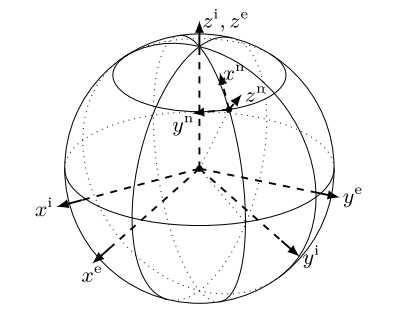
\includegraphics[width=0.47\textwidth]{Img/CoordinateFramesnei.png}}}%
%     \qquad
%     \subfloat[El marco \textit{s} del LIDAR dentro del robot móvil, y el marco \textit{b} en el centro de masa del mismo]{{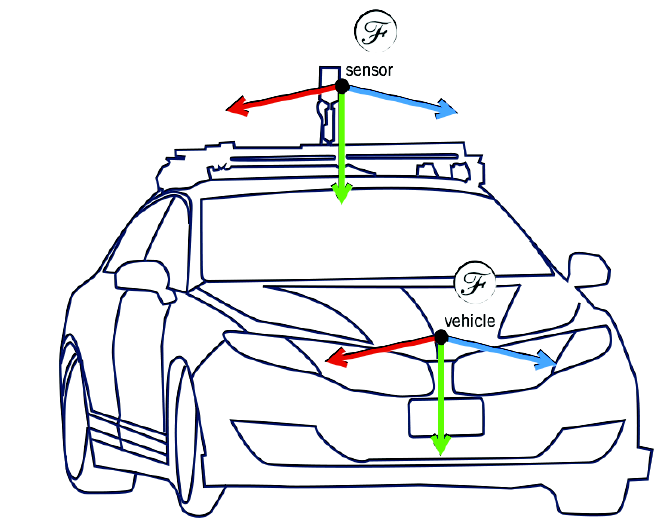
\includegraphics[width=0.47\textwidth]{Img/CoordinateFramesbs.png}}}%
%     \caption{Marcos de referencia presentados}
%     \label{fig:coordinateframes}
% \end{figure}
Con el fin de poder combinar todos los sensores a utilizar con sus respectivas referencias para formar la estimación de estado y el mapa, es necesario introducir una serie de marcos de coordenadas:
\begin{itemize}
    \item \textbf{Marco del vehículo (vehicle frame)$\undervec{\bm{\mathcal{F}}}_v$ o marco del cuerpo (body frame)} $\undervec{\bm{\mathcal{F}}}_b$: Es el marco de coordenadas del robot en movimiento. Su origen suele encontrarse en el centro de masa.
    \item \textbf{Marco sensorial (sensor frame)} $\undervec{\bm{\mathcal{F}}}_s$: Adjunto rígidamente a un sensor como, por ejemplo, el LIDAR, GPS o la unidad inercial de medición. Para localización, se suele ignorar la diferencia entre el el marco del robot móvil y el sensorial, ya que se asume que si se puede rastrear al sensor, es posible entonces rastrear cualquier punto en el robot móvil con la calibración adecuada.
    \item \textbf{Marco de navegación (navigation frame)} $\undervec{\bm{\mathcal{F}}}_n$: es un marco geográfico local en el que se quiere navegar. En otras palabras, es de interés en la posición y orientación del marco $\undervec{\bm{\mathcal{F}}}_v$ con respecto a este marco. Para la mayoría de las aplicaciones se define estacionaria con respecto a la Tierra. Sin embargo, en los casos en que se espera que el sensor se mueva a grandes distancias, se acostumbra mover y rotar el marco $\undervec{\bm{\mathcal{F}}}_n$ a lo largo de la superficie de la Tierra. Un marco de navegación típico es aquel que se encuentra adjunto a un punto de partida pertinente, y se encuentra alineado con el Norte, Este y Abajo (NED, de sus siglas en inglés).
    \item \textbf{Marco inercial (inertial frame)} $\undervec{\bm{\mathcal{F}}}_i$: Es un marco estacionario. La unidad inercial de medición, por ejemplo, mide la aceleración lineal y la velocidad angular con respecto a este marco. Su origen se encuentra en el centro de la Tierra y sus ejes $x$ e $y$ se encuentran fijos respecto a las estrellas distantes, mientras que el eje $z$ apunta al Norte verdadero. Esto quiere decir que, aunque la Tierra gire alrededor del eje $z$, los ejes $x$ e $y$ no se mueven.
    \item \textbf{Marco de la Tierra (Earth frame)} $\undervec{\bm{\mathcal{F}}}_e$: Coincide con el marco $\undervec{\bm{\mathcal{F}}}_i$, pero gira con la Tierra. Es decir, tiene su origen en el centro de la Tierra y los ejes que se fijan con respecto a la Tierra. En particular, el eje $x$ se alinea con el Ecuador, el eje $y$ está asociado a la regla de la mano derecha, y el eje $z$ apunta al Norte verdadero.
\end{itemize}

% Las coordenadas correspondientes a los marcos de la Tierra, de navegación e inercial pueden observarse en la Figura \ref{fig:coordinateframes}.a, mientras que las correspondientes al marco sensorial de, por ejemplo, un LIDAR, y al marco del vehículo se observan en la Figura \ref{fig:coordinateframes}.b. Estos serán de relevancia en las siguientes secciones.